\section{Z-Transformation}
\subsection{Konvergenzbereich}\script{S186}
Zum Konvergenzbereich (Region of Convergence) gehören alle komplexen z-Werte bei denen die z-Transformation einen endlichen Wert hat (keine Pole). Zu einer z-Transformation muss immer die ROC angegeben werden. Ist keine ROC angegeben wird angenommen, dass das Zeitsignal kausal war. Hat eine z-Transformation keine ROC, so existiert diese nicht!

\begin{align*}
	a^nu(n) &\transform \frac{1}{1 - az^{-1}} \qquad \text{ROC} = {\left. z \in \mathbb{C}\right| \left|z\right| \gt \left|a\right|} \\
	-a^nu(-n - 1) &\transform \frac{1}{1 - az^{-1}}  \qquad \text{ROC} = {\left. z \in \mathbb{C}\right| \left|z\right| \lt \left|a\right|} \\
\end{align*}
\begin{center}
	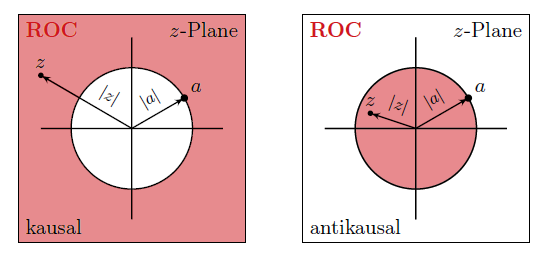
\includegraphics[width=\columnwidth]{Images/kausal_exmpale}
\end{center}

\subsection{Stabilität}
Alle Pole der $H(z)$ Funktion müssen \textbf{innerhalb} des Einheitskreis liegen. Für Grenzstabilität liegt der ROC genau auf dem Einheitskreis (Pol liegt auf dem Einheitskreis!)

\subsection{Frequenzgang}
Der Frequenzgang kann durch $\left.H(z)\right|_{z = e^{j\omega}}$ gezeichnet werden. Grafisch: Dem Einheitskreis in der Z-Ebene entlang fahren und die entsprechende Kontur ergibt den Frequenzgang.
\begin{center}
	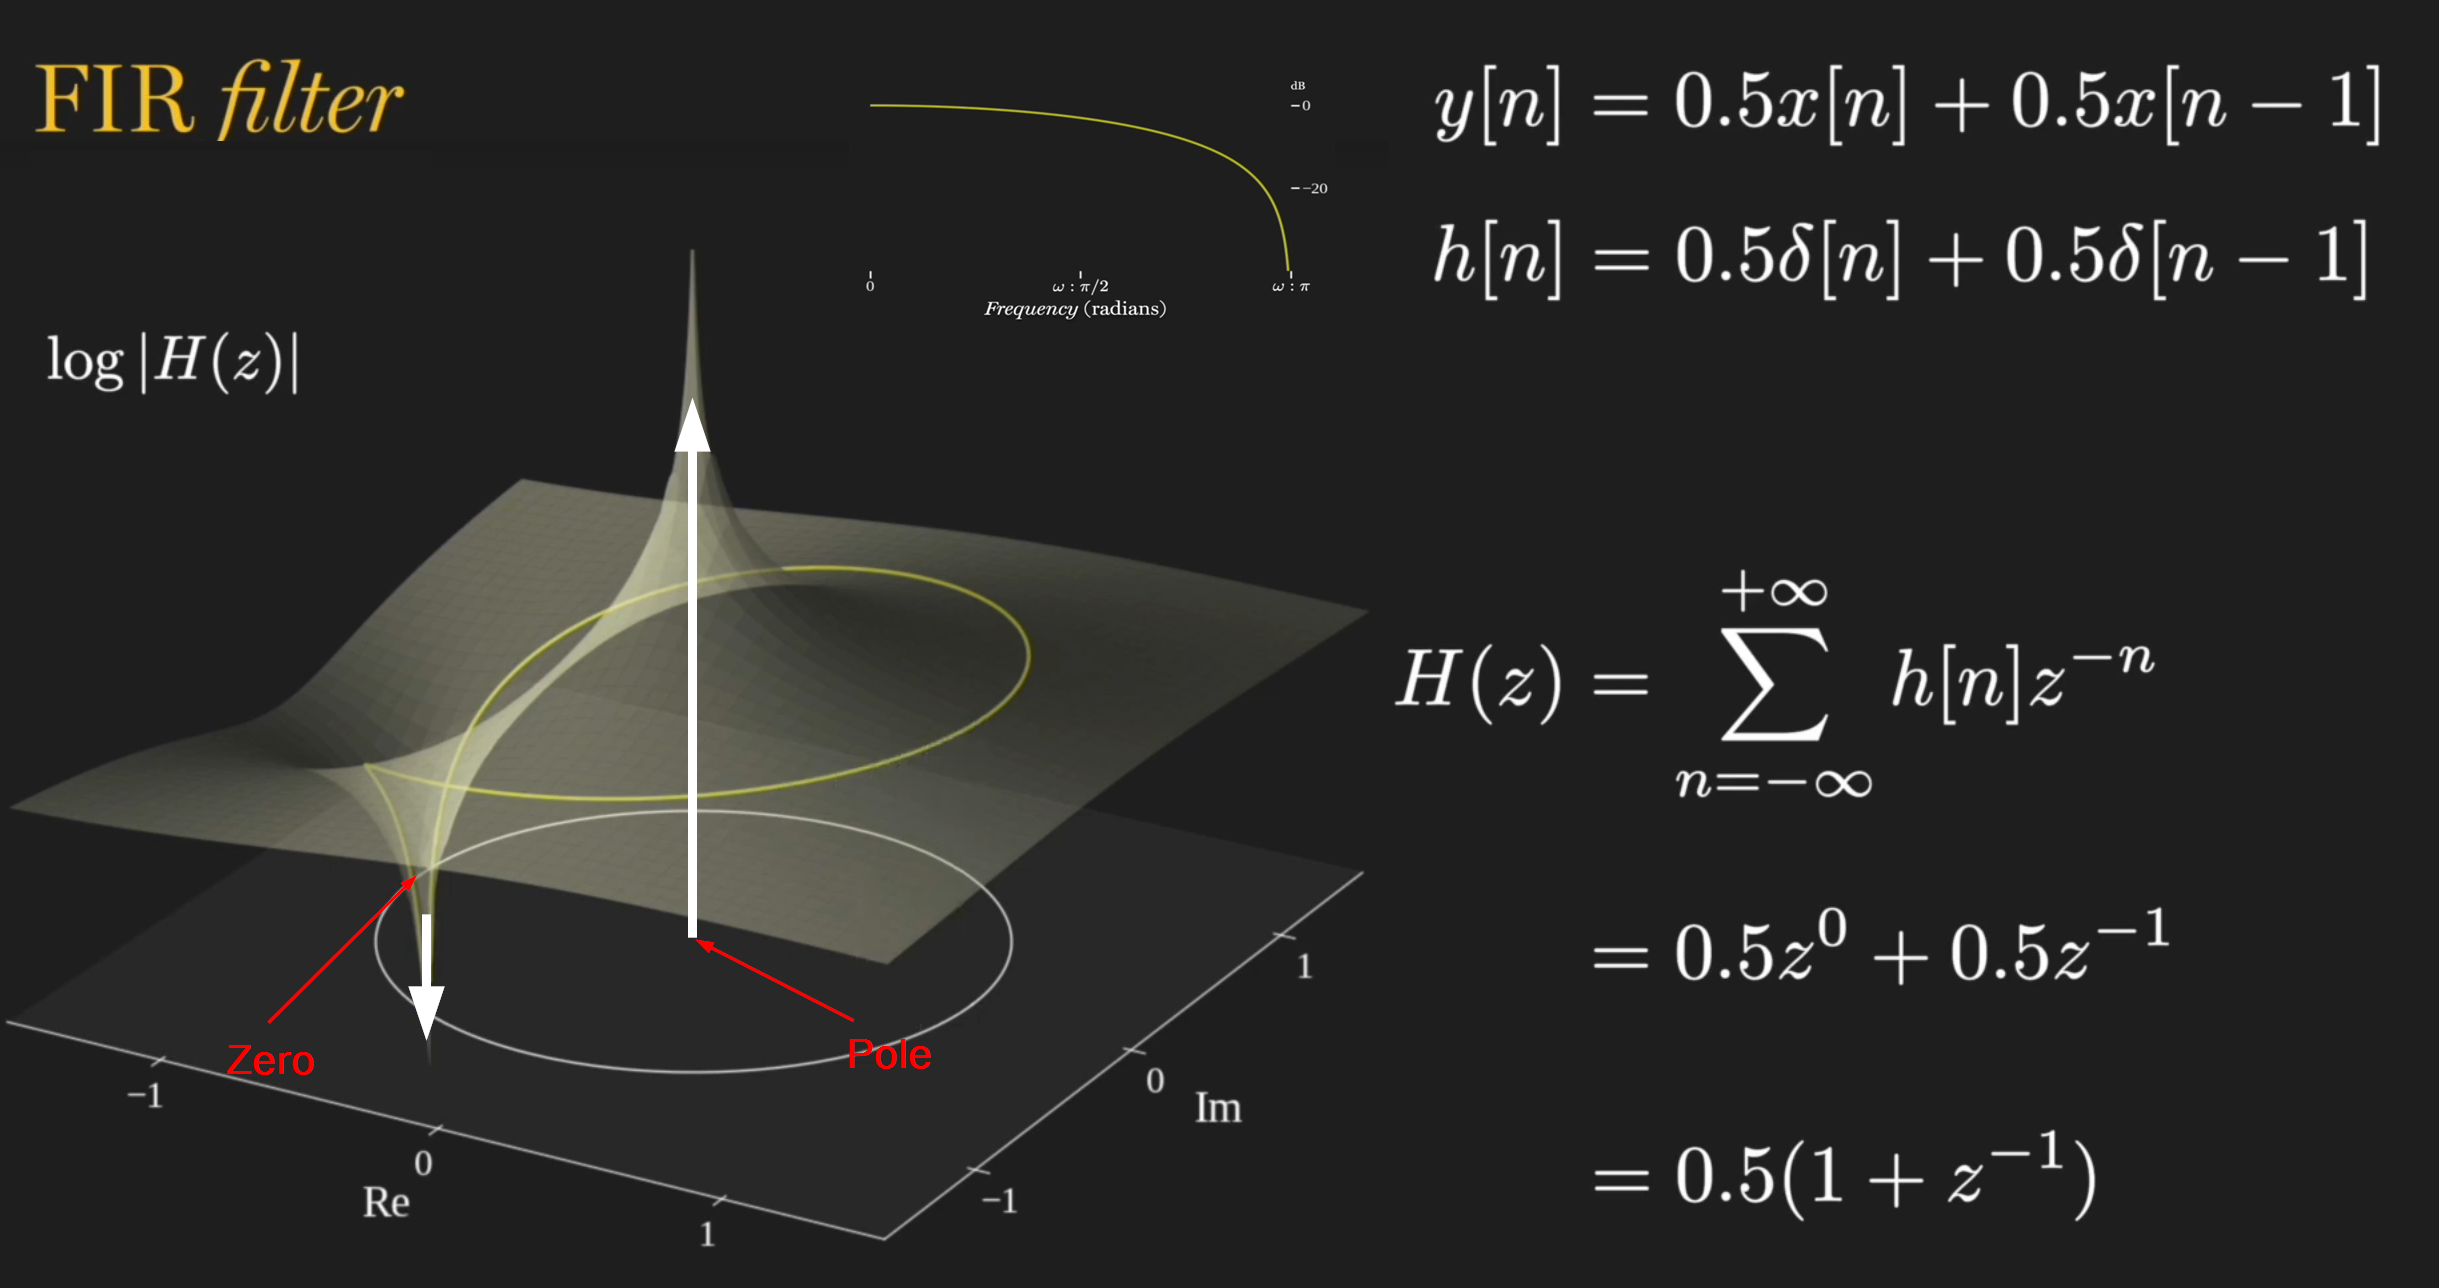
\includegraphics[width=\columnwidth]{Images/fir_example}
\end{center}


\textbf{Hinweis} für ein Pol $p_1$ und eine Nullstelle $z_1$:
\[
X(z)= \frac{1-z_1z^{-1}}{1-p_1z^{-1}} = \frac{z - z_1}{z - p_1}
\]
ergibt im Frequenzgang $X(\omega) = \left|x(\omega)\right|e^{j\arg X(\omega)}$:
\[
X(\omega) = \frac{e^{j\omega} - z_1}{e^{j\omega} - p_1}
\]

\textbf{Hinweis 2}: (gilt immer)
\[
\left|1 - a\cdot e^{-j\omega}\right| = \sqrt{1- 2a \cos(\omega) + a^2}
\]
\subsection{Inverse}\script{202}
Wenn $z^{-n}$ eine Div.0 ergibt, $X(z)$ mit $z^{+n}$ multiplizieren.
\begin{center}
	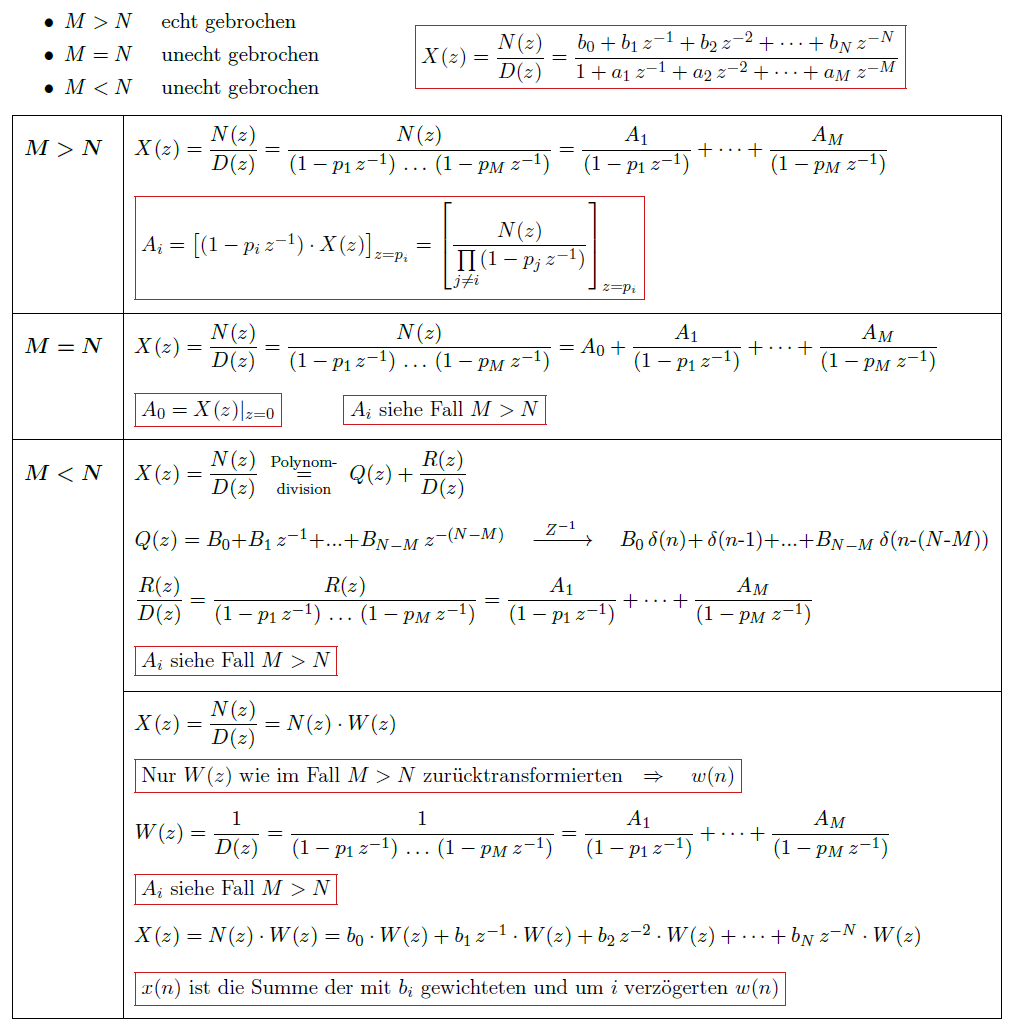
\includegraphics[width=\columnwidth]{Images/iztrans}
\end{center}
